\documentclass[journal]{IEEEtran}
\usepackage[utf8]{inputenc}

\usepackage{hyperref}
\usepackage{graphicx}
\usepackage{subfigure}

% typology diagrams
\usepackage{tikz}
\usetikzlibrary{shapes}

%tables
\usepackage{booktabs}
\usepackage{supertabular}
\usepackage{multirow}
\usepackage{varwidth}

\newcommand{\turn}[3][10em]{% \turn[<width>]{<angle>}{<stuff>}
  \rlap{\rotatebox{#2}{\begin{varwidth}[t]{#1}\bfseries#3\end{varwidth}}}%
  }
\usepackage{pdflscape} %% Used for very big table

\usepackage{paralist}

\usepackage[draft]{fixme}
\fxsetup{footnote}
\fxsetup{nomargin}

\graphicspath{{figs/}}

\newcommand{\ie}{{\textit{i.e.\ }}}
\newcommand{\cf}{{\textit{cf~}}}
\newcommand{\eg}{{\textit{e.g.\ }}}

\newcommand{\taxon}[2]{%
    \textbf{[#1] \emph{#2}}
}
\newcommand{\todo}[1]{\textbf{\textcolor{red}{TODO: #1}}}


% Macros related to concepts/statements typesetting
\newcommand{\concept}[1]{{\footnotesize \texttt{#1}}}
\newcommand{\stmt}[1]{{\footnotesize \tt $\langle$ #1\relax$\rangle$}}
\newcommand{\rawstmt}[1]{{\footnotesize \stmttt#1\relax}}
\def\stmttt#1 #2 #3\relax{{\tt#1} {\bf{\tt #2}} {\tt #3}}
\newcommand{\setstmt}[1]{{\footnotesize [\setstmttt#1\relax]}}
\def\setstmttt#1,#2\relax{\rawstmt{#1}, \rawstmt{#2}}

\title{Knowledge Representation for Service Robots: A Survey}
\author{Séverin Lemaignan, Moritz Tenorth, Rachid Alami, Michael Beetz}


\begin{document}

\maketitle


\begin{abstract}

The aim of this contribution is two-fold: we first propose a typology of
knowledge representation systems for service robotics that covers intrinsic
features like expressiveness or reasoning techniques as well as extrinsic
features like knowledge acquisition and integration into pre-existent robotic
architectures. We base the typology on an initial typical scenario of service
robotics.

We then survey the current knowledge representation system in the community to
identify which knowledge-bound cognitive abilities are today well understood
and implemented, and which would require more research efforts.

We hope this article may bring a clearer picture of the challenges of knowledge
representation and manipulation for the robotic research community.

\end{abstract}

\fxnote{Support material: \emph{What is a knowledge representation} by Davis,
Shrobe and Szolovits,
\url{http://groups.csail.mit.edu/medg/ftp/psz/k-rep.html}}


%%%%%%%%%%%%%%%%%%%%%%%%%%%%%%%%%%%%%%%%%%%%%%%%%%%%%%%%%%%%%%%%%%%%%%%%%%%%%%%%%%%%%%%%%%%
\section{Introduction}
\label{sect|intro}

\subsection{Knowledge as the Root of Cognitive Abilities}
\label{sect|cognitive-abilities}

The idea of \emph{Cognitive Robotics} was coined in the early 1990s by Reiter.
In a chapter on that subject in \emph{Foundations of Artificial
Intelligence}~\cite{Levesque2008}, Levesque reminds about the manifesto they
wrote together in 1998:

\begin{quotation}

    ``Central to this effort is to develop an understanding of the relationship
    between the knowledge, the perception, and the action of [\ldots] a robot. The
    sorts of questions we want to be able to answer are

    \begin{itemize} 

        \item to execute a program, what information does a robot need to have
        at the outset versus the information that it can acquire \emph{en route}
        by perceptual means?

        \item what does the robot need to know about its environment versus what
        need only be known by the designer?

        \item when should a robot use perception to find out if something is
        true as opposed to reasoning about what it knows was true in the past?

        \item when should the inner workings of an action be available to the
        robot for reasoning and when should the action be considered primitive
        or atomic?

    \end{itemize}

    and so on. With respect to robotics, our goal (like that of many in AI) is
    \emph{high-level robotic control}: develop a system that is capable of
    generating actions in the world that are appropriate as a function of some
    current set of beliefs and desires.''

\end{quotation}

To be answered, those questions have in common one prerequisite: the robot must
be able to manipulate \emph{explicitly} knowledge, and hence, need a way to
represent the knowledge.

This survey focuses on this knowledge representation issue: we aims at first
establishing a comprehensive typology of representational needs for
robotics in the specific context of service robotics, and then at painting the
current landscape of approaches to the knowledge representation problem in the
research community, in order to summarize the major trends and to identify the
possible shortcomings.

We have classified the features of knowledge representation systems (KRS) into
six broad categories: \emph{what can be represented?} or the
\emph{expressiveness} question ; \emph{how things are represented?} ; \emph{what
reasoning techniques are offered?} ; \emph{how knowledge is acquired and
anchored?} ; \emph{how the knowledge is made available and used by the other
components of the robot?} and \emph{which actual knowledge is stored?} or the
\emph{knowledge instantiation} question.

We have identified over ten projects that are either explicitly advertised as
knowledge representation systems or involve explicit knowledge manipulation
within a robot. By knowledge manipulation, we mean symbolic representation of
assertions, be it static statements on the world or spatio-temporal events, and
reasoning on this representation. Prominent features of each of these systems
illustrate how the various features of a knowledge representation system are
currently implemented.

We have also tried, for each project, to make clear \begin{inparaenum} \item
how informations from perception or interaction are turned into knowledge,
\item how, in return, symbolic concept are \emph{anchored} into the robot
sensori-motor space, \item how the knowledge representation system integrates
with the decisional layers of the robot, and how this can improve or ease
robotic control.\end{inparaenum}
\fxfatal{Do we really do it?}

\paragraph{What do we call ``knowledge''?}
\label{sect|on-knowledge}

Since we will discuss at length the concept of knowledge in the context of
robotics in the coming pages, it is useful to make our terminology explicit.

Be it in philosophy, cognitive sciences or computer sciences, reaching an
agreement on a definition of ``knowledge'' seems difficult.

Allen Newell's famous \emph{Knowledge Level}~\cite{Newell1981} can be a
starting point: for Newell, \emph{knowledge} is a medium between \emph{agents}
and \emph{goals}, \emph{actions}, \emph{bodies}. Whereas the symbol level deals
with representation, the knowledge level deals with language, semantics;
whereas the symbol level deals with inference, the knowledge level deals with
entailment. We will, at the conclusion of the article, give a second look to
this distinction.

In our robotic context, we define knowledge as a narrower concept, while
keeping Newell's link to actions: ``knowledge'' is for us  \emph{a set of
interrelated logical facts that are meaningful to the robot executive
controller}. By \emph{meaningful} we mean that can possibly be interpreted to
lead to a purposeful action. We will see that our main challenge while
designing a cognitive architecture is furthermore to make this knowledge as
\emph{explicit} as possible.

The relation of \emph{data} and \emph{information} to knowledge is a debated
epistemology question known as the ``DIKW'' hierarchy question. In this article,
we will associate data to low-level material like raw sensor output, and
information to uncontextualised symbolic facts.

To give a example, we can imagine a human reading a book while being tracked by
a Kinect sensor: the pose of the human skeleton in the world would be the data,
the fact \concept{looksAt(human, coords)} as interpreted by a geometric reasoning
module would be the information, the fact \concept{looksAt(john,
war\_and\_peace)}, fully grounded and connected to the whole knowledge base of
the robot would be proper knowledge.

\subsection*{Survey Inclusion Criteria}
\label{sect|inclusion-criteria}

Every robotic system has, implicitly or not, some knowledge representation
systems. It may range from a simple state vector to an explicit symbolic
knowledge base.  This survey focuses on the right end of this spectrum:
symbolic systems, suited for abstract reasoning.

Besides, we have decided to restraint the set of systems to those actually
implemented on robots, and used in semantic-rich environments (\ie dynamic,
partially unknown environments with a large range of different entities which
may have interactions). The typical scenario that would involve such robots is
a service robot in a human-friendly environment like a kitchen.

We have limited ourselves to systems that
\begin{inparaenum} 
    \item  run on \emph{service robot} (that is, robots that interact with 
    objects in a semantic-rich environment primarily designed for humans),
    \item  ground the knowledge in the physical world (physically embedded
    systems able to assess their environment),
    \item  are able to merge different knowledge modalities,
    \item  are able of on-line, dynamic knowledge acquisition and reasoning 
    (\ie not simple static databases).
\end{inparaenum}

These criteria exclude platforms like {\sc DyKnow}~\cite{Heintz2004}
which are focused on data fusion and knowledge grounding at lower levels.

We have also chosen not to include the GOLOG language and its
derivatives~\cite{levesque1997golog, Ferrein2008, Gspandl2011} in this survey. While
several implementations on robots, including service robots, do exist, the
focus of this language is on representation and reasoning about actions and
situations, and the link with symbolic, abstract knowledge is not explicit.

While classical cognitive architectures like {\sc Soar}~\cite{Lehman2006},
GLAIR~\cite{Shapiro2009} or {\sc ACT-R} have declarative knowledge
modules~\cite{Derbinsky2010} and have been recently used on service robots (see
{\sc ACT-R/E}~\cite{Kennedy2009} for instance), they are also absent from this
survey because we did not find much references in the literature on knowledge
manipulation and representation applied to real-world robotic scenarii for
these architectures.

A comprehensive reference on (bio-inspired) cognitive architectures is also
available from the BICA Society~\cite{BicaCogArch2011}.

\subsection{Previous work}
\label{sect|evaluation-literature}

The typology we propose is in part based on a comprehensive synthesis of
classifications and analysis found in the literature. This synthesis is focused
on cognitive abilities strictly related to knowledge manipulation in the
context of service robotics.

Levesque and Lakemeyer~\cite{Levesque2008} present in their chapter on
Cognitive Robotics several characteristics of knowledge representation systems
for robots, stressing the need of representing the \emph{dynamics of the
world}.  Sensing is included in the knowledge representation via
\emph{fluents}; they introduce the idea of \emph{possible worlds} to represent
distinct parallel mental models; action representation and reasoning about
tasks is discussed in the context of \emph{situation calculus}; \emph{open
world} vs. \emph{closed world} approaches are mentioned.  They also discuss how
robot programming and knowledge representation can be related. We integrate
most of these items in our typology.

In a slightly broader context, Heintz et al.~\cite{Heintz2008} define
\emph{knowledge processing middleware} as systems supporting ``declarative
specifications for flexible configuration and dynamic reconfiguration of
context dependent processing at many different levels of abstraction''. They
identify six characteristics: the system must be able to \emph{merge
informations} from different, possibly distributed sources; it should support
quantitative as well as qualitative processing of information, it should offer
\emph{bottom-up} and \emph{top-down} processing, it should be able to deal with
\emph{uncertainty}, allow for ``flexible configuration and reconfiguration''
(which require what we call here \emph{non-monotonicity}) and finally
\emph{meta-knowledge} and \emph{introspective capacities} (``declarative
specification of the processing functionalities'').

Several surveys compare global cognitive architectures \cite{Langley2006,
Vernon2007, Chong2009}. Langley, Laird and Rogers~\cite{Langley2006}
distinguish nine capabilities: recognition and categorisation, decision making,
perception and situation assessment, prediction and monitoring, planning,
reasoning, execution control, interaction and
learning/remembering/introspection. They also separately identify four
\emph{properties} of a cognitive architecture, that categorise how knowledge is
handled by the architecture: representation of knowledge, organisation of
knowledge, utilisation of knowledge and acquisition and refinement of
knowledge. This categorisation had a notable influence on our typology, and
many of these categories are also present in our proposal.

Vernon et al.~\cite{Vernon2007} split these architectures into two broad
categories: the \emph{cognitivist} ones (where cognition is considered as an
explicit computation problem, often based on symbol manipulation), and the
\emph{emergent} ones (where cognition only exists as a result of the
interaction of the system with its environment). The approaches presented in
this paper are, at a few exceptions, prototypical \emph{cognitivist} approaches
that aim at making knowledge explicit within the robot architecture. Vernon et
al. propose twelve \emph{characteristics of cognitive system} to compare
architectures. Amongst them, they mention the \emph{inter-agent epistemology}
(how the structure of the world is captured in a representation and shared),
the relation to \emph{embodiment}, the ability to \emph{anticipate} and to
\emph{adapt}, and the mechanisms of \emph{motivation}. While presented at the
level of the whole robotic architecture, these features also translate into
knowledge representation strategies and are relevant to our study.

Chong et al.~\cite{Chong2009} also provide a recent review of the main cognitive
architectures, with a focus on eight functions: perception, memory, goals
management, problem solving capabilities, planning, reasoning, learning and
links to neurobiology.

At an even broader scope, several authors from fields that are connected to
robotics have previously listed desirable features of artificial systems aiming
at rich cognitive abilities.

For instance McCarthy recently listed in~\cite{McCarthy2007} the challenges he
identifies on the road to a \emph{human-level AI}.

\begin{itemize}

	\item the ability to \emph{"operate successfully in the common sense
	informatic situation"},

	\item the necessity of relying on mathematical logic, as the most fruitful
	formalism for machine intelligence,

	\item the ability to deal with \emph{approximate concepts and approximate
	theories} (that would include representing them, and reasoning with them),

	\item non-monotonic reasoning,

	\item what McCarthy calls \emph{Elaboration Tolerance}: the ability to
	extend \emph{on demand} the closed domain of interpretation for a
	given assertion,

	\item the ability to formalise and reason about contexts,

	\item reasoning about events, and in particular, actions,

	\item the capacity of introspection,

	\item and finally, he points the issue of giving computer the right
	heuristics for decision making.

\end{itemize}

Coming from the perspective of natural language processing in situated context,
Roy and Reiter summarise in~\cite{Roy2005} what they see as the main challenges
to be tackled by knowledge representation systems: \emph{cross-modal
representation} systems, association of words with perceptual and action
categories (\emph{grounding}), modeling of \emph{context}, definition of the
right \emph{granularity} of models, integration of \emph{temporal modeling and
planning}, ability to \emph{match past (learned) experiences} with the current
interaction and ability to take into account the \emph{human perspective}.

Knowledge representation systems in robotics are directly affected by these
points, and we indeed integrate them in our typology, in slightly reformulated
ways.

\subsection{Article overview}
\label{sect|overview}

The paper is organized in three main sections.

Section~\ref{sect|krsoverview} gives a first broad overview of knowledge
representation in robotics. It introduces briefly a range of different
approaches that do not focus on a specific field of robotics, and instead
provide insights on the wealth of knowledge representation techniques available
to researchers.

Sections~\ref{sect|features} and~\ref{sect|surveyed-systems} then focus on eight
systems deployed on \emph{service robots}: Section~\ref{sect|features}
introduces a extensive typology of requirements and features of knowledge
representation systems, that we use as foundation to compare and evaluate the
systems we examine, and section~\ref{sect|surveyed-systems} then presents each
of the eight systems, and underlines their specificities.

We finally summarize in section~\ref{sect|conclusion} the current approaches and
we attempt to identify several research directions that are not sufficiently
addressed by the current state of the art.

%%%%%%%%%%%%%%%%%%%%%%%%%%%%%%%%%%%%%%%%%%%%%%%%%%%%%%%%%%%%%%%%%%%%%%%%%%%%%%%%
\section{Knowledge Representation in Robotics: an Overview}
\label{sect|krsoverview}

TDB

\todo{change wording, copied from other papers so far:}
\paragraph{Semantic maps}

Recent advances in object recognition however lead to more research on semantic
maps and thereby to a wider use of higher-level semantic knowledge in robotic
applications, though the ``level of semantics'' ranges from a  mere  classification
into different parts and object types~\cite{Rusu08RAS2} or the co-occurrence of
objects~\cite{vasudevan08} to environment representations in description
logic~\cite{zender2008conceptual}, statistical relational environment
models~\cite{limketkai05relational} and an embedding of spatial information
into an encyclopedic and common-sense knowledge base~\cite{tenorth10envmodel}.
The use of semantic maps as knowledge source for task planning has been
investigated by~\cite{galindo08taskplanning}. Other AI techniques that have
been used in robotics include the grounding of natural language in perception
and action \cite{Mavridis2006,kollar10natural}, planning of actions and
motions~\cite{wolfe10combined,kaelbling11planning}, and the generation of
robot controllers from logical constraints~\cite{kressgazit09planning}.

\paragraph{natural language understanding for direction following}
\cite{matuszek12commands}
\cite{duvallet13imitation}


\paragraph{(epsiodic) memories in robotics}

RACE \cite{rockel13ontology}
STRANDS?
CRAM$_m$ \cite{winkler13memory}

episodic memories in SOAR~\cite{nuxoll12episodic}

\paragraph{misc}
mining knowledge about object locations from the Web
\cite{zhou12webmining}



\todo{add something on the IEEE standard draft for a robotics and automation ontology}


% % % % % % % % % % % % % % % % % % % % % % % % % % % % % % % % % % % % % % % 
\section{Evaluation Criteria: A Typology of Knowledge Representation Requirements for Robotics}
\label{sect|features}

We propose to organize requirements from this imaginary cooking scenario where
numerous desirable features for a knowledge representation system for robotics
have been identified without any particular order.

This section proposes a more formal typology and a nomenclature of analysis
axis for a such a system. For each feature, we provide a short definition along
with links to relevant literature.

As previously mentioned, we propose six main categories, that cover both basic
and practical aspects: the formal
\taxon{A}{Expressiveness} of the system, the breadth and nature
of the \taxon{B}{Representations} allowed by the system, the
\taxon{C}{Reasoning} capabilities, how knowledge it acquired
\taxon{D}{Acquisition}, how the system integrates with the other components of
the robot sotware architecture \taxon{E}{Integration} and finally what we call
the knowledge \taxon{F}{Instantiation}, \ie the actual content of the knowledge
base.

The next paragraph details only briefly the exact meaning of these categories
and introduce accordingly sub-categories. We kindly refer the interested reader
to~\cite{lemaignan2012symbolic} for in-depth discussion of each of these
dimensions of knowledge representation systems, as well as related literature.

Table~\ref{table|contribution-by-systems}, at the end of the article, summarizes
the main contributions of each of the surveyed KRS with respect to these
dimensions.

\subsection{Expressiveness: What Can be Represented?}
\label{sect|expressiveness}

This first axis of analysis is its intrinsic expressive power. It answers the
question: what can be possibly represented. When it explicitly exists, the
\emph{language} of representation plays here an obvious role.

We subdivide the category \taxon{A}{Expressiveness} into five subcategories:
\taxon{A.1}{Logic formalism} classifies the underlying logical formalism of the
KRS (Horn clauses like for Prolog-based systems, Description
Logics~\cite{Baader2008}, Bayesian logics, etc.). \taxon{A.2}{Expressive Power}
quantifies the design choices made with respect to the actual expressive power
of the logical formalism: tradeoffs have to be found to allow both for high
expressiveness and tractable and decidable representations, and KRS authors
often add constraints on their representation logics to this end.
\taxon{A.3}{OWA/CWA} reflects the design choice between the \emph{open world}
(OWA) versus the \emph{closed world} (CWA) assumptions, which related to the
possibility of representing \emph{unknown} facts. \taxon{A.4}{Uncertainty}
relates to the ability for the system to represent both the \emph{intrinsic}
uncertainty of given facts, and the \emph{extrinsic} uncertainty due to
imperfect perception by the robot. \taxon{A.4}{} relates only to the possibility
of \emph{representation}. Reasoning on uncertain facts is discussed in
\taxon{C.4}{}. The last features of a KRS related to representation is
\taxon{A.5}{Meta-cognition} that conveys the capability for a system to
represent and exhibit it own internal structures and representation mechanisms.

%%%%%%%%%%
\subsection{How things are represented?}
\label{sect|higher-level-domain-representation}

This category focuses on questions that involve
representational challenges (time, space, context) or require specific
cognitive capabilities (theory of mind, introspection, memory).

The dimension \taxon{B.1}{Roles}, with its sub-categories \taxon{B.1.1}{Space},
\taxon{B.1.2}{Time} and \taxon{B.1.3}{Actions}, deals with the approaches that
the KRS suggests to represent these three important \emph{roles} in robotics
(spatial relations, time and representation of actions). To give a few examples
(in no way exhaustive), \emph{Spatial relations} covers techniques like
topological maps, allocentric and egocentric frame projections. \emph{Time
representation} includes Allen's interval algebra~\cite{Allen1984}, Ghallab's
chronicles~\cite{Ghallab1996} or the concept of \emph{fluent}. \emph{Actions}
concern themselves with representation of \emph{pre-, post-conditions},
\emph{thematic roles} or \emph{plans}.

\taxon{B.2}{Context} describes if and how a given KRS represents the
\emph{interpretation frame} of the situation and its own knowledge. This is
often related to the initial \emph{common-sense knowledge} available to the
robot. \taxon{B.3}{Modality} refers to the ability, for the KRS, to represent
possible alternate worlds or belief states. A typical application of a
\emph{modal} knowledge model is the implementation of a \emph{theory of mind},
\ie an independent belief model for the other agents the robot interact with.
\taxon{B.4}{Introspection} covers both \emph{self-knowledge} (what do I know
about myself?) and a weaker version focused on the explicit representation and
reasoning on the \emph{robot's own skills} (can I execute a given task?).
Finally, \taxon{B.5}{Memory} refers to the implementation of
different kind of bio-inspired memory models like \emph{declarative},
\emph{procedural} or \emph{episodic}, and the attached processes
(\emph{forgetting}, \emph{selectively remembering}, etc.).

%%%%%%%%%%
\subsection{Reasoning techniques}
\label{sect|reasoning}

As one can expect, many reasoning techniques born in artificial intelligence
have found their place in robotics over the years. We propose to consider ten
subcategories of \taxon{C}{Reasoning} that reflects in our opinion important
features in regards to the general requirements of robotics (like decision
making being tractable in pseudo-real time, being able to deal with partially
unknown or uncertain domain or specific reasoning related to interaction with
the physical world).

Again, the descriptions of these ten subcategories hereafter are very
superficial. Readers can refer to~\cite{lemaignan2012symbolic} for the details.

\taxon{C.1}{Standard reasoning} covers conventional reasoning techniques based
on logical inferences (for instance, \emph{forward/backward chaining} or
\emph{semantic tableaux}). The main problems that these techniques address are
\emph{concept satisfiability}, \emph{consistency checking} and \emph{instance
checking}. \taxon{C.2}{Instantiation and structural alteration} describes how
dynamic a system is with respect to its internal knowledge structure (allowing
for modification of the knowledge structure, often called \emph{TBox}, may
impact the capability for the system to \emph{learn} for instance).
\taxon{C.3}{Lazy evaluation} describes the ability for a KRS to delay active
knowledge acquisition or reasoning operations until the value is actually
needed, and may have a strong impact on the overall scalability of the system.
\taxon{C.4}{Uncertainty} groups all the features related to reasoning over
uncertain knowledge (like probabilistic inference).
\taxon{C.5}{Non-monotonicity} discusses how systems deal with non-monotonic
inferences, \ie exceptions to a rule or inferences that lead to the retractation
of previously inferred facts. Techniques to deal with non-monotonic reasoning
include for instance \emph{Default Logics}.  \taxon{C.6}{Presupposition
accomodation} is the ability for a system to automatically create a context
allowing to make sense of a proposition. This is tighly linked to the capability
for a system to deal with \emph{under-specification}. \taxon{C.7}{Prediction and
explanation} (with subcategories \taxon{C.7.1}{Projection},
\taxon{C.7.2}{Legality}, \taxon{C.7.3}{Diagnosis} and
\taxon{C.7.4}{Explanation}) relates to the capabilites for a system to predict
and project the outcomes of a sequence of actions onto the logical system, and
conversely, to justify and explain the sequence of entailments that lead to a
conclusion. Related to this category, \taxon{C.8}{Planning} discusses to which
extend a KRS can be used for \emph{symbolic task planning}, \ie the ability for
a robot to select a sequence of actions in order to reach a given final state.
\taxon{C.9}{Physics-based reasoning} describes the capability for a symbolic
knowledge representation system to rely on physical reasoning (which may include
geometry, dynamics, collision checking, etc.) to derive symbolic inferences.
Finally, \taxon{C.10}{Learning} groups the various capabilities that lead to
learning behaviours.

%%%%%%%%%%%%%%%%%
\subsection{Acquiring knowledge}

In the survey inclusion criteria, we have chosen to only consider robotic
systems that acquire knowledge by themselves, at runtime. The category
\taxon{D}{Acquisition} reviews the different approaches to knowledge acquisition
and semantics extraction. \taxon{D.1}{Acquisition and fusion} examines the
techniques to first acquire new logical statements and then \emph{align} them to
the corpus already available to the robot. Depending on the source of knowledge,
we distinguish three further subcategories: \taxon{D.1.1}{Sensing} covers the
techniques that translate perceptions into symbolic knowledge,
\taxon{D.1.2}{Interaction} focuses on knowledge specifically stemming from
interaction (typically, language processing), and \taxon{D.1.3}{Linked
Resources} relates to the connections and alignement issues with external
(often Web-based) knowledge bases.

\taxon{D.2}{Grounding} discusses the KRS capabilities in regards to attaching a
practical meaning to the symbol it manipulates. In the context of robotics, it
mainly consists in building and maintaining a bi-directional link between
sub-symbolic representations (sensors data, low-level actuation) and symbolic
representations.

Finally, \taxon{D.3}{Instrinsic Motivation} describes the possible
\emph{internal} mechanisms by which the robot seeks by itself to acquire more
knowledge.


%%%%%%%%%%%%%%%%%
\subsection{Practical integration in robotic architectures}
\label{sect|integration-robot}

Knowledge representation systems have limited usefulness for robotics if they are
considered in isolation, and it seems important to also evaluate KRS from the
perspective their integration into larger control architectures that includes
perception routines, decision-making processes and actuation control.
\emph{Practical} integration also suggests to take into account real-world
constraints, like performances and monitoring tools that come along with the KRS.

\taxon{E}{Integration} is hence subdivided: The integration of the KRS with the
\taxon{E.1}{Sensori-motor} layers may adopt various paradigms (from passive
\emph{semantic blackboards} to active KRS that directly query the sub-symbolic
layers. \taxon{E.2}{Executive layers} examines conversely how the KRS is used
from the perspective of the robot controller. Here also, many different
approaches have been investigated, from classical server-client architecture, to
DSL-like language extensions. \taxon{E.3}{Monitoring} details the support tools
provided by the system for the developpers to monitor and introspect their
system. This is especially important for knowledge representation systems
because they often lie at the heart of the architecture, and act as hubs for
many other components. \taxon{E.4}{Performances}, finally, evaluates the
performances of the KRS, both in term of scalability and classification speed
\taxon{E.4.1}{Raw performances}, and in term of cognitive abilities provided by
the system \taxon{E.4.2}{Cognitive performances}. Note that performances of KRS
are notoriously difficult to assess since on one hand, cognitive architectures
for robotics are often build upon tightly interleaved modules which makes it
difficult to test a KRS in isolation, and on the other hand, we lack standard
benchmarks and scales for cognitive capabilities.

%%%%%%%%%%%%%%%%%%%%%%%%%%
\subsection{Knowledge instantiation}

The last category of our taxonomy looks at the actual \emph{content} of the
knowledge base: the knowledge instantiation. Here, \emph{instantiation} does
not only refer to the instantiation of the knowledge structure (what we have
called the ABox), but also includes the knowledge structure itself (the TBox).

The \taxon{F.1}{Design strategy} of the KRS can be \emph{top-down} (from an
initial symbolic model down to the percepts), \emph{bottom-up} or  a mix of
both. The bottom-up and top-down strategies reflect how the knowledge structure
itself is constructed: either from generic categories, typically extracted from
standard upper-ontologies or by successive classification and refinement of
percepts.

\taxon{F.2}{Common-sense and alignment} discusses if and how the KRS reuse
existing pools of knowledge like \emph{upper-ontologies}, and how the question
of knowledge \emph{alignment} is handled. \taxon{F.3}{Metrics and quality
criteria} includes qualitative and quantitative metrics that give an insight on
the size, complexity and effectiveness of knowledge base available to the robot.
These metrics include for instance the number of terms and assertions, but also
the type of predicates that are used, or the computed Description Logics
expressiveness (when applicable).  Qualitative evaluation of ontologies is a
research field in its own right, and introduce criteria like \emph{accuracy,
adaptability, clarity, completeness, computational efficiency, conciseness,
consistency}. The last category is \taxon{F.4}{Granularity}, that accounts for
the level of details considered in the knowledge representation system, that can
go down to storing SIFT features~\cite{Suh2007} directly in the KRS.

%%%%%%%%%%%%%%%%%%%%%%%%%%%%%%%%%%%%%%%%%%%%%%%%%%%%%%%%%%%%%%%%%%%%%%%%%%%%%%%%%%%%%%%%%%%
\section{Existing systems for knowledge representation in service robotics}
\label{sect|surveyed-systems}

Table \ref{table|surveyed-systems} lists the knowledge representation
systems that we have surveyed.

This section briefly presents each of them.

\begin{table*}\scriptsize
\begin{center}

\begin{tabular}{p{2.2cm}p{1.6cm}p{4cm}p{2.4cm}p{3.4cm}p{1.5cm}}
\toprule
{\bf Project} & {\bf Category} & {\bf Authors (Institution)} & {\bf Programming language} & {\bf Knowledge model/Logical Formalism} & Main reference \\
\midrule
ARMAR/Tapas & Formal & Holzapfel, Waibel \par (Karlsruhe TH) & & TFS (Typed Feature Structures) & \cite{Holzapfel2008}\\
CAST Proxies & Ubiquitous & Wyatt, Hawes, Jacobsson, Kruijff (Brimingham Univ.,
DFKI Saarbrücken) & & Amodal proxies & \cite{jacobsson2008crossmodal} \\
GSM & Structural & Mavridis, Roy \par (MIT MediaLab) & & & \cite{Mavridis2006} \\
Ke Jia Project & Formal & Chen et al. \par (Univ. of Science and Technology of China) & ASP (Answer Set Programming) & ASP & \cite{Chen2010} \\
{\sc KnowRob} & Formal & Tenorth, Beetz \par (TU Munich) & {\sc Prolog} & {\sc Prolog} + OWL-DL &  \cite{Tenorth2009a} \\
NKRL & Language & Zarri et al. \par (Paris Est Créteil Univ.) & NKRL & & \cite{Sabri2011} \\
%OBOC & KRS & Mendoza & & & & & \cite{Mendoza2005} \\
ORO & Formal & Lemaignan, Alami \par (LAAS-CNRS) & {\sc Java} & OWL-DL ({\sc Jena}) + {\sc Pellet} & \cite{Lemaignan2010} \\
OUR-K/OMRKF & Formal & Lim, Suh et al. \par (Hanyang Univ.) & ? & DL + Horn Clauses &  \cite{Lim2011, Suh2007} \\
PEIS KR\&R & Formal & Daoutis, Coradeshi, Loutfi, Saffiotti \par (Örebro Univ.) & {\sc C}, {\sc CycL} & CycL (1st and 2nd order logics, modal logics) & \cite{Daoutis2009} \\
%Golog & Language & Levesque (Toronto Univ.) & & {\sc Prolog} & & & \\
% & & Varadarajan, Vincze \par (TU Wien) & & & & & \cite{Varadarajan2011} \\ % -> affordances, but no implementation on a robot
% & & Kaelbling, Lozano-Pérez \par (MIT CSAIL) & & & & & \cite{Kaelbling2011} \\ % -> mostly planning under uncertainty
% & & Hertzberg (Osnabrück Univ.) \\ % -> affordances, semantic mapping
% (based on {\sc KnowRob} & & (JSK) \\

\bottomrule

\end{tabular}
\end{center}

\caption{List of surveyed systems. Categories are \emph{Formal} for systems
that have a formal underlying knowledge representation, \emph{Ubiquitous} for
systems where knowledge is fully distributed, \emph{Language} for languages
used as KRS on robots or \emph{Structural} for KRS where knowledge is
represented as special data structures.}

\label{table|surveyed-systems}
\end{table*}

%\fxfatal{Bielefeld -> could not find much\ldots}
%\fxfatal{Kollar/Tellex -> really focusing on the natural language grounding}

\subsection{ARMAR/Tapas}

{\sc Tapas} is the name of the knowledge representation system and dialogue
manager found on the ARMAR~III robot~\cite{Holzapfel2008} for the Karlsruhe
Institute of Technology.

Knowledge in {\sc Tapas} exists as procedural knowledge (plans) and declarative
knowledge. The later is split into \emph{lexical knowledge}, \emph{semantic
knowledge} and a database of identified objects (with their properties). The
\emph{lexical knowledge} contains lexical and grammatical informations about
the objects. The \emph{semantic knowledge} is organised into an ontology
relying on \emph{typed feature structures} (TFS~\cite{Carpenter1992}, a
formalism originating from the computational linguistics community, and a
superset of first-order logic).

{\sc Tapas} has a strong focus on natural language grounding. It proceeds by
generating grammars from properties represented in the ontology to parse and
understand dialogue.

Another focus is put on handling unknown words and objects. {\sc Tapas}
provides routines to recognise unknown entities, and propose and interactive
and iterative verbal process to categorise (including adding new categories)
those new concepts.

\paragraph{Experiments} {\sc Tapas} has been used experimentally in a kitchen
environment where naive users had to ask the robot for an object and get
information about another object.

\subsection{CAST knowledge model}
\label{sect|cast}

CAS (\emph{CoSy Architecture Schema}) Toolkit~\cite{Hawes2007} is a
comprehensive toolkit aimed at building cognitive architectures for robots
through a set of interconnected \emph{SA} (\emph{subarchitectures}). The CAS
does not expose a central knowledge base as seen in other works. It represents
instead knowledge as unrooted \emph{proxies}. Those proxies are formally
defined in \cite{jacobsson2008crossmodal} as $p= \langle F_p, u_p \rangle$ where $F_p$ is
a set of instantiated features (like $\phi^{Colour}_{red}$) and $u_p$ a
\emph{proxies union} that form an equivalence class corresponding to one
entity.

A union of proxies forms a global amodal representation of an entity, that can
be explicitly shared and manipulated. Being not centralised, the knowledge
model can be qualified of \emph{ubiquitous}. Furthermore, knowledge source in
the CAS architecture is tightly bound to the on-line grounding process (be it
grounded in perception or in dialogue). While nothing seems to prevent it, no
{\it a priori} knowledge (including common-sense knowledge) is used.

Knowledge sharing is ensured by the event mechanism of CAST: modules can
monitor proxies for alteration by other modules. Jacobsson et al. mention how
this can apply to reinforcement learning: the vision module creates a proxy for
an orange object. This proxy get monitored by a learning module. In parallel,
the proxy is bound to an union by the natural language understanding module
that add new a feature like \emph{"this object is a fruit"}. The learning
module is called back, and can add this new information to its model.

In the presented implementation, the CAST knowledge model does no allow for
effectively representing actions or temporal information.\fxwarning{What about
reasoning? can they retrieve for example 'all proxies for colorful objects'?}

\paragraph{Knowledge Acquisition} Several techniques for knowledge acquisition
have been explored within the CAST framework. Cross-modal knowledge
fusion~\cite{Hawes2007a} is well studied, and the interaction with natural
language processing~\cite{Kruijff2010, Kruijff2010a} is a particular emphasise
of the project.

In~\cite{Hawes2011}, Hawes et al. also explore \emph{curiosity} mechanisms in
the context of spatial representations with the robot \emph{Dora}.

\paragraph{Experiments} CAST has been used in several experiments, including
table-top manipulation (with a focus on language understanding) and more
recently on the Dora robot~\cite{Hawes2011} for indoor exploration.

\subsection{GSM}
\label{sect|gsm}

GSM (for \emph{Grounded Situation Model})~\cite{Mavridis2006} is a knowledge
representation system primarily built to ``facilitate cross-modal
interoperability'',  especially in the context of verbal interaction with a
robot.

GSM does not rely on any formal language but rather on a layered data structure
(figure~\ref{fig|gsm}) that organises the surrounding world into agents and
relations between agents.  Each agent (any animate or inanimate object) is
attached to a physical model (made of \emph{body parts} that have properties
like their position, color, etc.) and a mental model (which is a recursively
embedded GSM, thus allowing a sort of theory of mind).

\begin{figure}
    \centering
    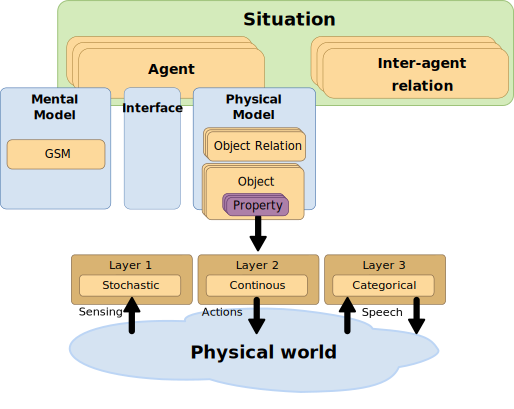
\includegraphics[width=0.9\columnwidth]{gsm.pdf}

    \caption{Simplified hierarchical structure of the Grounded Situation Model,
    based on~\cite{Mavridis2006}.}

    \label{fig|gsm}
\end{figure}

Properties are represented in three layers: a stochastic representation, close
to sensory percepts, a \emph{continuous single-valued} encoding of the
stochastic model, and a discrete, categorical model.

One notable feature of GSM is the \emph{bidirectionality} of the grounding
process: not only sensor percepts are abstracted into categories suitable for
human conversation, but human utterance (like ``There is a red ball in the
center of the table'') can also be turned into property descriptions. This
basically enable the knowledge representation system of the robot to
\emph{imagine} entities.

GSM also features several strategies for managing time and events.
\emph{Moments} are created by storing timestamped snap-shots of GSM, and
\emph{event classifiers} allow to define and detect events.

\paragraph{Experiments} GSM has mostly been tested on table-top manipulation
and interaction tasks (a ``conversational helping hand'' as stated by the
authors) implemented on a 7-DOF arm equipped with force feedback, cameras for blob
tracking and speech recognition (Sphinx4). Mavridis and Roy provide in addition
an in-depth analysis of the performance of GSM by the mean of a standard
psycholinguistic test, the \emph{Token test}~\cite{DiSimoni1978}.

\subsection{Ke Jia Project}
\label{sect|kejia}

The Ke Jia project~\cite{Chen2010} integrates on a mobile platform a knowledge
representation language with natural language processing, task planning and
motion planning.

Knowledge representation relies on \emph{Action Language C}, itself based on
\emph{Answer Set Programming} (ASP)~\cite{Gelfond2008}. These languages, that
are syntactically close to Prolog, are based on \emph{stable models} of logic
programs, and support non-monotonic reasoning. Default and non-monotonic
reasoning has been especially researched within the Ke Jia project for symbolic
task planning~\cite{Ji2011} and underspecified natural language processing.

Amongst other features, the natural language processing capabilities of the
system support acquisition of new logical rules at run-time.

\paragraph{Experiments} The Ke Jia robot has been demonstrated in several tasks
involving human-robot interaction with natural language. These tasks include a
task with multiple \emph{pick \& carry} that are globally optimised, naive
physics reasoning via taught rules or more complex scenarii with the robot
delivering drinks, taking into account changing and mutually exclusive
preferences of users.


\subsection{KnowRob}
\label{sect|knowrob}


{\sc KnowRob}~\cite{Tenorth2009a} is an integrated knowledge management system
developed at the Technical University of Munich. It is build as a set of
modules (figure~\ref{fig|knowrob} organised around a core reasoning system
written in Prolog. This core module interfaces through Java/Prolog or
C/Prolog APIs with external modules.

\begin{figure}
    \centering
    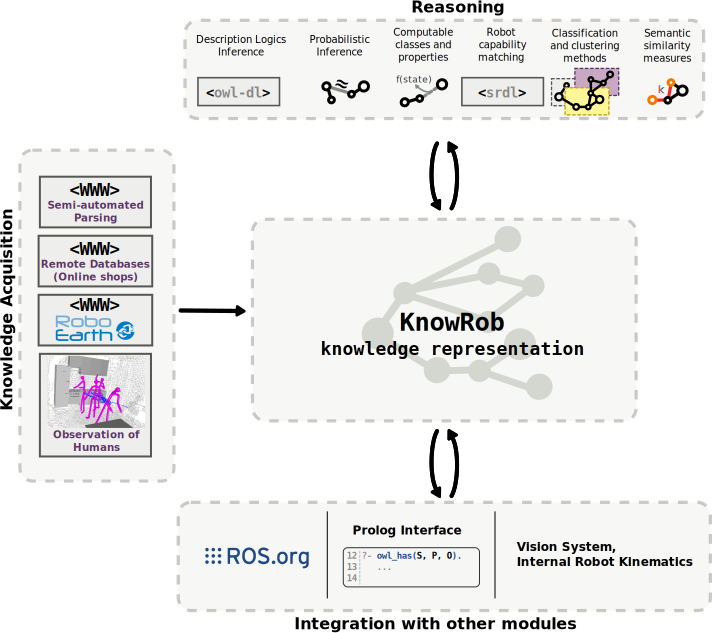
\includegraphics[width=0.7\columnwidth]{knowrob.pdf}

    \caption{Overview of the {\sc KnowRob} framework, taken
    from~\cite{Tenorth2011}.}

    \label{fig|knowrob}
\end{figure}

Extension modules can plug into the system to provide specialised reasoning
capabilities or interfaces to external data sources, \eg to read object
detections from the vision system. These modules operate on the level of
instances (ABox).

\paragraph{Knowledge model} {\sc KnowRob} can load OWL ontologies, and the
\emph{KnowRob-Base} ontology is provided as a common-sense ontology, with a
focus on household and kitchen domains. {\sc KnowRob} also store and reason on
introspective knowledge through the \emph{Semantic Robot Description
Language}~\cite{Kunze2011} that allow to represent symbolically the
capabilities of the robot, and is used for planning.


\paragraph{Reasoning Techniques} Amongst the notable {\sc KnowRob} extensions,
{\sc ProbCog}~\cite{Jain2009} is an effort to provide probabilistic reasoning
based on bayesian networks, integration with naive physics reasoning has been
studied~\cite{Kunze2011a}, automatic parsing of Web resources in semi-natural
language has been also experimented with~\cite{Nyga2009}.

\paragraph{Grounding} {\sc KnowRob} offers a mechanism called \emph{computables} that allow to
evaluate certain predicates by calling external dedicated functions (for
instance, the valuation of a proposition like \stmt{object1 isOn object2} is
computed when required by calling a specific geometric reasoning module). In
combination with Prolog's lazy evaluation strategy, this supports a good
scalability.

Computables rely on various subsystem to evaluate. In particular, it relies on
the CoP framework~\cite{Klank2009} and \emph{semantic maps}~\cite{Blodow2011}
for the recognition of objects and environment.

%\paragraph{Integration with Decisional Layers} CRAM~\cite{Beetz2010}

\paragraph{Experiments} {\sc KnowRob} has been deployed on several scenarii at
the Technical University of Munich, on the PR2 robot and on a 2-arm custom
mobile manipulator in the scope of the ``assistive kitchen''~\cite{Beetz2008}
project. These experiments include retrieval and automated parsing of recipies
from the Web, retrieval and manipulation of various kitchen tools, cooperation
between two robots.

\subsection{NKRL}
\label{sect|nkrl}

\emph{NKRL} stands for \emph{Narrative Knowledge Representation Language}.
While this language is developed since a long time by Zarri~\cite{Zarri1997,
Zarri2008}, recent research direction include application to the robotic
field~\cite{Sabri2011}. NKRL is not {\it per-se} a knowledge representation
system, as it is primarily a language. However, it is used as the
representation and reasoning mechanism for robots by Sabri et al.

\paragraph{Knowledge representation} The NKRL language semantics are stored in
two ontologies: an ontology of concepts $\Omega$ and an ontology of events
$\Psi$. The ontology of events is made of action or situation templates.
Templates are a set of predicates (MOVE, PRODUCE, RECEIVE, EXPERIENCE, BEHAVE,
OWN and EXIST) associated to thematic roles. Grounding and reasoning with NKRL
is based on template matching.

\paragraph{Experiments} The main scenario of development for NKRL-based robots
is the Smart Home and monitoring of eldery people. Knowledge acquisition
partially rely on ambient intelligence (RFID, pressure sensors in the chairs,
etc.). The scenario is still being implementated.

\subsection{OUR-K and OMRKF}
\label{sect|omrkf}

The Ontology-based Unified Robot Knowledge~\cite{Lim2011} (OUR-K) framework,
successor of the Ontology-based Multi-layered Robot Knowledge
Framework~\cite{Suh2007} (OMRKF), is a knowledge representation system based on
five inter-related \emph{classes} of knowledge (figure~\ref{fig|omrkf}). It
proposes a layered approach to knowledge representation that allows to
integrate the grounding process to the knowledge representation process. OUR-K
knowledge model is implemented with a mix of Description Logics for the concept
hierarchies and Horn clauses.

\begin{figure}
    \centering
    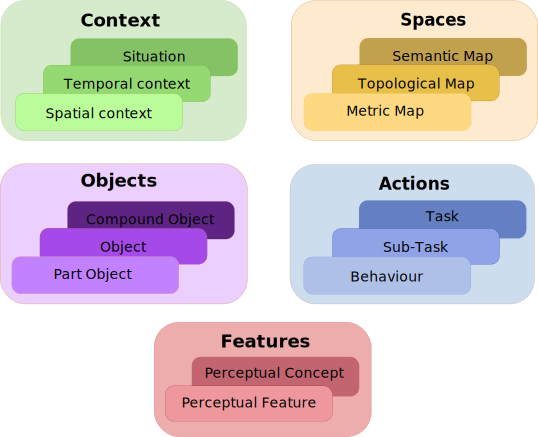
\includegraphics[width=0.8\columnwidth]{ourk.pdf}

    \caption{OUR-K organises knowledge into fives \emph{classes}, each composed
    of \emph{levels}. Figure based on~\cite{Lim2011}.}

    \label{fig|omrkf}
\end{figure}

Each level of knowledge is build as three stages of ontological realization: a
\emph{meta-concept} (the level itself, like ``temporal context'', ``behaviour''
or ``object feature''), a taxonomy of concepts inside this level (for instance
$cup : Object \sqsubseteq tableware : Object$) and an instantiation of the
taxonomy ($cup1 : cup$).

\paragraph{Representation} The environment is represented in OUR-K in the
$spaces : Model$ knowledge level as a classical three layers mapping (metric,
topological and semantic maps). Objects (in $objects : Model$) are localised in
$spaces : Model$ through Voronoi nodes.

The knowledge class $Context$ proposes an explicit statement of spatial context
(mostly geometric relations between objects), temporal context and a more
general \emph{high-level} context, inferred from spatial and temporal contexts.

Finally, the $Activity$ knowledge class store compound actions in a HTN-like
structure, exploited at run-time by a planner.

\fxwarning{re-read the paper to improve the section...}

\paragraph{Experiments} Experiments conducted with OUR-K and OMRKF include
finding kitchen objects and reporting about their state to a human.  This
experiment also shows how OUR-K can deal with objects only partially matched by
their descriptor by introducing a $candidate()$ function.

\subsection{ORO}
\label{sect|oro}

\begin{figure}
    \centering
    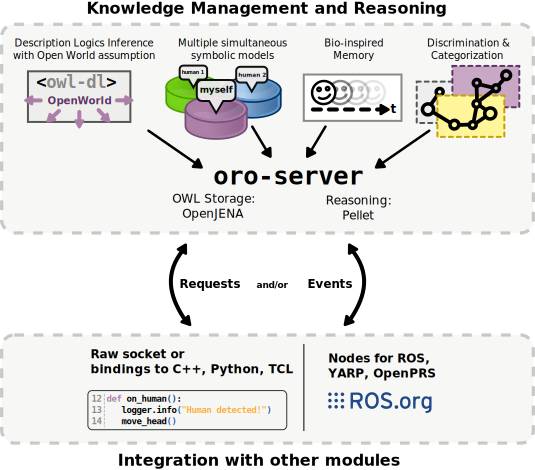
\includegraphics[scale=0.36]{oro.pdf}

    \caption{Overview of the ORO server, taken from~\cite{Lemaignan2012}.}

    \label{fig|oro}
\end{figure}

\subsection{PEIS KR\&R}
\label{sect|peis-ecology}

{\sc PEIS Ecology}~\cite{Saffiotti2005} is a software \emph{ecosystem} that aim
to binds autonomous robotics with ambient intelligence (network of sensors).
\emph{PEIS} stands for \emph{Physically Embedded Intelligent System}: every
robots or intelligent device in the environment is abstracted as a PEIS.

Each PEIS physical component is running a \emph{PEIS Kernel} instance.
Communication between instance relies on a custom P2P communication protocol.

The PEIS architecture allows for adding new abilities through software
components sharing the common \emph{tuple space}.

We consider here the semantic layer~\cite{Daoutis2009}, referred as \emph{PEIS
KR\&R}, that includes symbolic representation and reasoning.

\fxwarning{have a look to latest Daoutis paper!}

% More in details:
% - object identification based on viewpoint independent SIFT features
% - formalised anchoring system that explicitly match percieved attributes to predicates
% - Cyc predicates
% - ground 12 colors, based on a paper on color perception. Could be useful for us.
% - idem, they cite a paper on what spatial relations to compute
% - location of objects based on a previously provided semantic map (but not much on this semantic map)
% - two "memories": the robot memory stores the current list of percieved objects ; the archive memory stores what is not percieved anymore
% - uses directly Cyc (ie, 250 000 common sense concepts\ldots), via CycL language -> 2nd and higher order logics (quantification over predicates, functions, etc)
% Remark: using 2nd order logic (ie meta statements), it would be easy to store the knowledge of each agent
% - disambiguation in concept name by asking human to decide amongst all concepts known by Cyc
% - template based natural language
% - experiment conducted in a "smart" indoor environmement + simple robot

\paragraph{Knowledge model} The PEIS Knowledge representation system relies on
the {\sc ResearchCyc} and {\sc CycL} language to represent knowledge. The {\sc CycL} language
allows to represent first order logic sentences and has extensions for modal logics and higher order logics.

\fxwarning{Is modal logics and higher order logics actually used in PEIS?} 

As a system relying on {\sc CycL}, contexts can be expressed as
\emph{microtheories}: the truth or falsity of a set of statement depends of the
\emph{microtheory} in which these statements are evaluated.

\fxwarning{OWA/CWA?}

\begin{figure}
	\centering
	\includegraphics[width=0.9\columnwidth]{peis-architecture.pdf}
	\caption{The PEIS knowledge representation system, taken from~\cite{Daoutis2009}}
	\label{fig|peis-archi}
\end{figure}

The PEIS KR\&R system is deeply integrated to the general PEIS Ecology
\emph{smart} environment. Figure~\ref{fig|peis-archi} gives an overview of the
interactions between PEIS knowledge processing layers.

\paragraph{Knowledge Acquisition} The primary source for knowledge acquisition
is perception.  The PEIS ecosystem provides a SIFT-based object recogniser used
in conjunction with ceiling cameras for object localisation.  Other perceptual
modalities are available (like human tracking, ambient environment monitoring).

A template-based natural language parsing system may also be used to add new
assertions to the system.

The system can ask the human for help to disambiguate between concept names.

\paragraph{Anchoring} Daoutis et al. formalise the issue of anchoring as
finding a \emph{predicate grounding relation} $g \subseteq \mathcal{P} \times
\Phi \times D(\Phi)$, where $\mathcal{P}$ is a set of predicate symbols, $\Phi$
a set of percept's attributes, and $D(\Phi)$ the domain of these attributes.

In the current implementation, object category (returned by the SIFT
classifier), color, location, spatial relations (both topological -- \emph{at},
\emph{near} -- and relative to the robot -- \emph{left}, \emph{behind}, etc.)
and visibility are the five classes of extracted attributes.

\paragraph{Integration in the robot architecture}
\label{sect|peis-integration}

The PEIS framework offers through the \emph{PEIS middleware} a practical way to
insert a new component into the shared \emph{tuple space}.  Thus, the KR\&R
module can be seamlessly integrated into the PEIS ecosystem.

\paragraph{Experiments} Experiments involving PEIS take place in a Smart Home
environment (\emph{PEIS Home}). The implemented case studies explore
dialogue-based interaction with the robot about known objects.

%%%%%%%%%%%%%%%%%%%%%%%%%%%%%%%%%%%%%%%%%%%%%%%%%%%%%%%%%%%%%%%%%%%%%%%%%%%%%%%

%%%%%%%%%%%%%%%%%%%%%%%%%%%%%%%%%%%%%%%%%%%%%%%%%%%%%%%%%%%%%%%%%%%%%%%%%%%%%%%%%%%%%%%%%%%%
\section{Synthesis: How Current Systems Tackle the Knowledge Representation
Challenge?}
\label{sect|conclusion}

This section summarizes the different approaches to knowledge representation and
reasoning that are surveyed in the previous section, and attempt to identify
research perspectives.

First, the Table~\ref{table|contribution-by-systems} presents, system by system
and feature by feature, a landscape of current research, underlining the main
design choices and scientific \emph{contribution} of each of the KRS that we
have examined.

Then, we go over again the nine ``challenges'' proposed by McCarthy and Roy (see
section~\ref{sect|evaluation-literature}) to evaluate how far we are on the road
to natural interaction and, to slightly paraphrase McCarthy, ``human-level
robots''.

\subsection{Logic formalisms, continuous world}

McCarthy underlines the necessity of relying on mathematical logic, as the most
fruitful formalism for machine intelligence. This is largely the case. Almost
all the systems we have surveyed rely on logical formalisms, in several cases
as a mix of declarative languages (often based on Decription Logics) and
logical programming languages (Prolog, expectedly, but not only).

The two exceptions (the CAST knowledge model and GSM) are however 
interesting: CAST proposes a pervasive model of knowledge that is convincing from
the grounding perspective (but likely suboptimal for deliberative tasks), and
GSM encodes knowledge in an amodal (continuous, geometric) model while
preserving features that are usually specific of symbolic models (like theory
of mind or categorical knowledge).

The interleaving of discrete symbolic models with the continuous physics of the
world remains a major challenge, and techniques vary a lot: besides the CAST
proxies and the GSM amodal model, most systems directly extract physical
attributes of the environment to insert them in the symbolic model ({\sc Tapas},
Ke Jia, OUR-K, PEIS), thus skipping altogether an intermediate geometric model.
ORO has tight (but unidirectional) links with an intermediate geometric
representation (called {\sc Spark}), and {\sc KnowRob} adopt a top-down approach
where local geometric models are set up on-demand to compute symbolic properties
like relative locations.

\subsection{Management of uncertainty and approximation}

McCarthy also mentions the necessity to deal with \emph{approximate concepts
and approximate theories} (that includes representing them and reasoning with
them).

The most notable attempt at modeling uncertainty down to the knowledge
representation is {\sc ProgCog}, an extension of {\sc KnowRob}. Theoretical
and practical performances issues (including decidability) remain however
difficult to overcome.

It can be also noted that some effort do exist to provided probabilistic
reasoning to Description Logics based systems (like the {\sc Pronto}
reasoner~\cite{Klinov2008}), but this does not appear to be a major focus in the
currently available tools.


\begin{landscape}
\begin{table}\tiny
\begin{center}
\begin{tabular}{p{0.2cm}p{3.4cm}p{1.6cm}p{1.3cm}p{1.7cm}p{1.5cm}p{2cm}p{2cm}p{2cm}p{1.4cm}p{1.8cm}}
\toprule
\multicolumn{2}{c}{\bf Category}                                                     & ARMAR \cite{Holzapfel2008}& CAST \cite{Hawes2007}       & GSM \cite{Mavridis2006}     & {\sc Ke Jia} \cite{Chen2010}& {\sc KnowRob} \cite{Tenorth2009a}  & NKRL \cite{Sabri2011}                           & ORO \cite{Lemaignan2010}                      & OUR-K \cite{Lim2011}          & PEIS \cite{Daoutis2009}        \\
                                                                                                                                                                                                                                                                                                                                                                                                                   
\midrule                                                                                                                                                                                                                                                                                                                                                                                                           
                                                                                                                                                                                                                                                                                                                                                                                                                   
\multirow{4}{*}{\turn{90}{\bf Expressiveness}}                   & Logical formalism & TFS                       & (none)                      & (none)                      & ASP                         & Prolog                             & NKRL language (FOL + 2nd order extensions)      & DL (OWL)                                      & DL + Horn clauses             & {\sc CycL}                     \\
                                                                           & OWA/CWA &                           &                             &                             & CWA                         & CWA                                &                                                 & OWA                                           &                               &                                \\
                                                              & Modeling uncertainty &                           &                             & ++ (stochastic models)      &                             & {\it+++} ({\it ProbCog} \cite{Jain2009}) & +                                         &                                               & + (\emph{candidate} entities) &                                \\
                                                                    & Meta-cognition &                           &                             &                             &                             & +                                  & + (transformation rules)                        & ++ (reification, taxonomy walking)            &                               &                                \\
\hline                                                                                                                                                                                                                                                                                                                                                                                                             
\multirow{7}{*}{\turn{90}{\bf Representation}}                & Space Representation &                           &                             &                             &                             &                                    &                                                 & ++ ({\em perspective-aware symbolic locations} \cite{Sisbot2011})& ++         &                               \\
                                                               & Time representation &                           &                             & ++ (snapshots)              &                             & + (Allen's intervals, via \emph{computables} & ++ (event oriented)                   &                                               & +                             &                                \\
                                                                    & Actions/Events &                           &                             & ++ (events classifiers)     &                             & ++ (action recognition \cite{Beetz2010a})  & +++ (everything is an event)            &                                               & +++                           &                                \\
                                                                           & Context &                           &                             &                             &                             &                                    & ++ (template matching)                          &                                               & ++                            & ++ (microtheories)             \\
                                                                          & Modality &                           &                             & ++ (recursive model)        &                             &                                    &                                                 & ++ (Theory of Mind \cite{Warnier2012a})       &                               &                                \\
                                                                    & Self-knowledge &                           &                             &                             &                             & + (SRDF \cite{Kunze2011})          &                                                 &                                               &                               &                                \\
                                                                     & Memory models &                           &                             &                             &                             &                                    &                                                 & +                                             &                               & +                              \\
\hline                                                                                                                                                                                                                                                                                                                                                                                                             
\multirow{9}{*}{\turn{90}{\bf Reasoning}}                   & Standard FOL reasoning &                           &                             &                             & +++                         & +++                                & + (template matching)                           & ++                                            & +                             & ++                             \\
                                            & Instantiation and structure alteration & ++                        &                             &                             & ++                          & + (dynamic instantiation)          &                                                 & ++ (TBox alteration)                          &                               &                                \\
                                                                   & Lazy evaluation &                           &                             &                             &                             & +++ (Prolog, computables)          &                                                 &                                               &                               &                                \\
                                                           & Non-monotonic reasoning &                           & ++ \cite{Hawes2011}         &                             & +++ \cite{Ji2011}           & + \cite{Tenorth2012}               &                                                 &                                               &                               &                                \\
                                                      & Presupposition accommodation &                           &                             & +++                         &                             &                                    &                                                 &                                               &                               &                                \\
                                    & Prediction, projection, diagnosis, explanation &                           &                             &                             &                             & + \cite{Tenorth2012}                                   & ++                                              & + (explanation)                               &                               &                                \\
                                                                     & Task planning &                           &                             &                             & ++ \cite{Ji2011}            & +                                  &                                                 & +++ ({\em HATP})                              & +                             & {\it++}                        \\
                                                           & Physics-based reasoning &                           &                             &                             & +                           & {\it+++} ({\em naive physics \cite{Kunze2011a}}) &                                   &                                               &                               &                                \\
%                                                                         & Learning & ++                        & ++ \cite{Jacobsson2008}     &                             &                             &                                    &                                                 &                                               &                               &                                \\
\hline                                                                                                                                                                                                                                                                                                                                                                                                             
\multirow{5}{*}{\turn{90}{\bf Acquisition}}                         & Cross-modality & + (pointing gestures)     & ++                          & +++ (amodal model)          &                             &                                    &                                                 & ++                                            &                               & ++ ({\em ambient intelligence})\\
                                                                               & NLP & +++                       & +++ \cite{Kruijff2010a}     & +++                         & +++                         &                                    &                                                 & +++ ({\em Dialogs} \cite{Lemaignan2011a})     &                               & + (template-based)             \\
                                                                     & Web Resources &                           &                             &                             &                             & {\it+++} ({\em Web content processing \cite{Nyga2009}})&                             &                                               &                               &                                \\
                                                                         & Grounding &                           & ++                          & ++ (bidirectional)          &                             & +++ ({\em semantic maps \cite{Blodow2011, Klank2009}}) &                             & ++ ({\em amodal model} \cite{Lemaignan2012})  & +++ (bottom-up)               & +++ \cite{Loutfi2008}          \\
                                                              & Intrinsic Motivation &                           & ++ \cite{Hawes2011}         &                             &                             &                                    &                                                 &                                               &                               &                                \\
\hline                                                                                                                                                                                                                                                                                                                                                                                                             
\multirow{4}{*}{\turn{90}{\bf Integration}}     &   \ldots with sensori-motor layers &                           &                             & +                           &                             & +++ (computables, local geometric models) &                                          &                                               & +                             & ++ (tuple space)               \\
                                                      & \ldots with executive layers &                           & ++ (ubiquitous events)      & +                           &                             & ++ (language extensions) \cite{Beetz2010} &                                          & ++ (semantic events)                          & ++                            & ++ (tuple space)               \\
                                                          & Monitoring and debugging &                           &                             &                             &                             & +(Prolog tracer, visualisations...)&                                                 & + ({\em remote visualisation})                &                               &                                \\
                                                           & Performances evaluation &                           & ++ \cite{Hawes2008}         & ++ (Token test)             & +                           & + \cite{Tenorth2011}               &                                                 &                                               &                               &                                \\

\bottomrule

%\end{tabularx}
\end{tabular}
\end{center}

\caption{Design choices and main domains of contribution of current KRS (+
indicates \emph{moderate contribution}, +++ indicates \emph{major
contribution}). Italics mean that the feature is implemented as an external
module. Main references are given in the table header. When relevant,
feature-specific publications have been provided.  An empty cell means that
either the system has no specific focus on this domain or we could not find
relevant literature.}

\label{table|contribution-by-systems}
\end{table}
\end{landscape}

\subsection{Non-monotonic reasoning}

McCarthy gives a particular importance to non-monotonic reasoning. Systems like
Ke Jia explicitly tackle this issue.

A monotonic system does not theoretically allow for knowledge retraction during
the reasoning, which is an important issue in the robotic context where the
world model is likely to be often altered.  However it is a practical issue
only if the reasoning process has to be \emph{continuous} during the whole
robot's activity lifespan, which is rarely the case. It is often possible to
stop the reasoner, alter the knowledge, and restart the inference process on a
new domain.

Non-monotonicity can also be partially dealt with with appropriate time
representation and reasoning (the reasoner then only takes into account
statements that are set as valid for a given moment) or with dedicated reasoners
for tasks requiring non-monotonic reasoning like symbolic task planning
\fxwarning{mention ORO + HATP}.

Finally, probabilistic reasoning also implicitly leads to non-monotonic
reasoning, by relying on a continuous description of the state of the
world.

Non-monotonicity is however of broader significance to the knowledge
representation field, in particular for the representation of common-sense
knowledge where \emph{default} representation is currently sorely lacking.

It is also related to what McCarthy calls \emph{elaboration tolerance}: the
ability to extend \emph{on demand} the closed domain of interpretation for a
given assertion, to take into account new contextual knowledge.

\subsection{Modeling of contexts}

Both Roy and McCarthy mention the importance of formalizing and reasoning about
contexts. Many of the KRS we have surveyed mention at some point the context
modeling, but no consistent interpretation, let alone theory, of context
management has clearly emerged.

Several approaches for building contextualized knowledge have been however
hinted in section~\ref{sect|features}: symbolic environment interpretation,
perspective taking and independent mental state for each agent, grounded natural
language resolution, self-awareness of its own activity. Much remains to be done
for a robot to actually identify its current context as well as contexts that
may be referred to.

\subsection{Reasoning about time, events and actions}

While representation of spatial roles (topology, placement, with or without
perspective-taking) is well studied and KRS usually integrate with spatial
perception and reasoning components, time representation and integration in
knowledge systems is less uniform.

The two main tasks that require time reasoning are task planning and sequence
recognition (in particular, action recognition). Systems that directly
integrate task planning (like OUR-K, {\sc KnowRob}) thus have mechanisms (like
fluents in {\sc KnowRob}) to represent time.

Other approaches include storing snapshots of the knowledge state (like GSM),
that is used to move back to past mental states (of the robot or of another
agent).

Integration of these techniques with memory mechanisms (forgetting and
reinforcement learning) remains mostly to be explored.

Regarding events, several systems (GSM, NKRL, ORO) have adopted an {\em
event-oriented} architecture where conditions (or templates) are used to
trigger decisional and execution processes.

\subsection{Grounding in a multi-modal environment}

Symbol grounding remains a focus for most of the developers of cognitive
architectures for robots, and all the systems we have surveyed implement
grounding strategies. Most of the systems
adapt their grounding strategies to the sensing modality, so that grounding can
not be considered as a single, well delimited process.

Some systems (ORO, GSM) introduce an intermediate step in the grounding process
by the mean of an amodal model of the environment that aggregates the
perceptions (or suppositions) in a single place. This enables geometric
reasoning that takes into account all the perceptual modalities (typically
required for spatial perspective taking: we need to know where the humans are
looking at, and also where are the objects), and also improve the observability
of the system.

We note in addition that the development of high-level sensors is simplifying
the grounding task. The most obvious example is the human tracking system
provided with the low-cost Kinect family of devices, and now used
pervasively in the robotics lab. Not only this system segments and computes the
pose of humans that enter its field of view, but it also tracks them (including
in case they are partially or completely occluded). This kind of high level
sensing device does not completely remove the need of grounding one symbolic
instance of a human with the physical human, but the task is much simpler than
it used to be.

Many systems also tackle the difficult question of natural language processing.
The CAST middleware, in particular, has been used in the European CoSy and CogX
projects as knowledge base by linguists~\cite{Kruijff2010a}. This demonstrates
the interest for the grounding of verbal interaction within the cognitive
robotics community, and we are likely to reach important milestones in this
field in the coming years.

Merging more modalities (especially, back-channel communication, deictic
gestures and social gazes) also sparks a lot of attention, and is becoming more
and more present as symbolic knowledge available to the control layers.

\subsection{Common-sense}

McCarthy actually starts his list by affirming that intelligent systems must be
able to \emph{``operate successfully in the common sense informatic
situation''}. This question of the \emph{common-sense} is probably one of the
toughest because what \emph{common-sense} mean is not very clear at first place
(since, by definition, common-sense is, well, common-sense...). We feel,
however, that it is related to a diffuse cultural background, and one may even
claim that, for a system to acquire common-sense reasoning is equivalent to
solve the strong AI challenge (this is at least more or less McCarthy's opinion).

Knowledge representation systems have usually a pragmatic approach to
common-sense: they reuse knowledge bases stored on the Web. While {\sc KnowRob}
is the only one explicitly working on common-sense reasoning, through
physics-based reasoning, integration with Web databases or parsing of
semi-structured Web documents), several other KRS rely on Web standards (OWL,
OpenCyc) to represent their knowledge (Table~\ref{table|knowledge-sources} lists
the sources of common-sense knowledge found in the surveyed systems). With the
development of initiatives like OpenMind that encode with the same standards
common-sense facts and rules, there is a strong potential for our robot to gain
common-sense knowledge from well-structured online resources in the coming
years.

%%%%%%%%%% Underlying knowledge model table %%%%%%%%
\begin{table}
\begin{center}

\begin{tabular}{lp{4cm}}
\toprule
{\bf Project} & {\bf Common-sense \par knowledge source} \\
\midrule
{\sc KnowRob} & {\sc OpenCyc}, processed web content, custom OWL-DL ontology \\
ORO & {\sc OpenCyc}, custom OWL-DL ontology \\
PEIS Ecology & {\sc ResearchCyc} \\
NKLR &  None \\
CAST Proxies &  None \\
GSM &  Predefined categories \\
OUR-K & {\it A priori} knowledge structure and axioms, custom set of instances\\
Ke Jia & None \\
ARMAR/{\sc Tapas} & Custom ontology related to the kitchen\\

\bottomrule

\end{tabular}
\end{center}
\caption{Underlying knowledge sources for each project}
\label{table|knowledge-sources}
\end{table}

\subsection{Learning, representation of experience, introspection}

Learning at the level of the knowledge representation system has been explored
in conjunction with visual perception systems (mentioned for instance for the
CAST project~\cite{jacobsson2008crossmodal}). {\sc KnowRob}, by filling its pool of
facts from informations automatically extracted from the Web~\cite{Nyga2009},
can also be considered as a \emph{learning} system (it autonomously acquire
knowledge). We lack however a formal study of learning strategies and
techniques at the knowledge representation level.

Representation and matching of past experience is a related topic. This ability
is a key step for general action recognition, and is of particular importance
for the robot to assess the state of the interaction with the human.

While we already mentioned that several systems are able to reason on past
states, we are not aware of existing implementation of algorithms to reflect on
past experiences.

This is itself related to introspection and meta-cognition: the shift towards
explicit knowledge representation exemplified in the nine systems we have
presented, has a major impact on the meta-cognitive capabilities of our robots.
They can exhibit, manipulate and reason on their internal belief state (what we
will call in the conclusion the \emph{cognitive observability}). We have still
to discover all the possibilities that are open by this important cognitive
ability.

\subsection{Perspective-awareness}

Finally, Roy mentions \emph{the ability to take into account the human
perspective}: this cognitive ability, that relates to the representation of
different modalities, is explicitly advertised in ORO and GSM only: ORO
explicits the perspectives in different symbolic mental states while GSM
recursively stores models for each agent.  We think however that several of the
other systems could easily gain support for alternative belief models, leading
the way to becoming perspective-aware KRS.

\subsection{Conclusion: the Future Directions to Explore}

TDB

%%%%%%%%%%%%%%%%%%%%%%%%%%%%%%%%%%%%%%%%%%%%%%%%%%%%%%%%%%%%%%%%%%%%%%%%%% 
\section*{Acknowledgements} 

%%%%%%%%%%%%%%%%%%%%%%%%%%%%%%%%%%%%%%%%%%%%%%%%%%%%%%%%%%%%%%%%%%%%%%%%%% 

\bibliographystyle{ieeetr}
\bibliography{biblio}


\end{document}
